\section{\secsubgraphiso}
\label{sec_subgraph_isomorphic}

There are many different ways to draw a graph.  Suppose that you and I each draw a graph and our graph drawings look different.  How do we know if our graphs are actually the same graph (isomorphic)?  For example, are any of the graphs $G_1$, $G_2$, and $G_3$ drawn in \Cref{fig_G1G2G3} the same (isomorphic)? 

    \begin{figure}[hbtp]
        \centering
        \input{Tikz/isomorphic_opening}
        \caption{Are any of the graphs $G_1$, $G_2$, $G_3$ isomorphic?}
        \label{fig_G1G2G3}
    \end{figure}    

Recognizing when two apparently different objects are, for all mathematical purposes, the same or different is a powerful skill.  For example, suppose that we are modeling a problem and encounter a new graph $G$, a graph that we know nothing about.  But then we realize that $G$ is isomorphic to a graph $H$ that we know well.  Then everything that is true about the known graph $H$ is automatically true for the new graph $G$ as well.  The concept of isomorphic occurs throughout mathematics.  

There is no known efficient algorithm for determining if two graphs are isomorphic.  We begin this section with a visualization tool that can help and close this section by introducing vocabulary about graphs that live within other graphs (subgraphs), which can also offer clues about whether two graphs are isomorphic.

%%%%%%%%%%%%%%%%%%%%

\newcommand{\subplanarity}{Planarity}
\subsection{\subplanarity}
\label{sub_planarity}

When we draw a graph, it is acceptable to have edges that cross each other.  Any point of intersection of those edges in the drawing is \emph{not} a vertex.  For example, the complete graph $K_5$ is typically drawn with many edges crossing, as in \Cref{fig_K5}.

\begin{figure}
    \centering
    %Used in \Cref{sec_subgraph_isomorphic}

% K5
    \begin{tikzpicture}
        [scale =.5]
        \GraphInit[vstyle=Welsh]
        \SetGraphUnit{2}
        \SetVertexNoLabel
        \Vertices{circle}{$B$,$A$,$E$,$D$,$C$}
        \Edges($A$, $B$, $C$, $D$, $E$, $A$)
        \Edges($A$, $C$, $E$, $B$, $D$, $A$)
    \end{tikzpicture}
    \caption{The standard drawing of the complete graph $K_5$ with many edges crossing.}
    \label{fig_K5}
\end{figure}

In some situations, we might prefer to draw a graph without edges crossing. For example, if the graph were modeling a physical system, such as train tracks or electrical wires, we might want to avoid edge crossings, or at least find a drawing with as few edge crossings as possible.  It is reasonable to ask whether a graph can be drawn without crossings.  For example, can you find a way to draw $K_5$ without any edge crossings?

We formalize this idea with a definition.

\begin{defn}[Planar graph]
\label{defn_planar}
~
    \begin{apart}
        \item An \vocab{edge crossing} in the drawing of a graph is a point of intersection of two edges other than at a vertex.
        \item A graph is \vocab{planar} if it can be drawn in the plane without any edge crossings.  For example, consider the graph $G$ drawn in \Cref{fig_four_drawings_K4_minus_edge}.  In the fourth drawing of $G$, the edges $\{3,4\}$ and $\{1,2\}$ cross, but no edges cross in the first three drawings of $G$. Thus, $G$ is planar.
        \item A graph is \vocab{nonplanar} if it cannot be drawn in the plane without any edge crossings.  For example, it turns out that the complete graph $K_5$ is nonplanar.
        \end{apart}
    \end{defn}

Let's look at an activity redrawing planar graphs without edge crossings.  

\begin{act}[Planarity puzzle]
\label{act_planarity_puzzle}
~    
    \begin{apart}
        \item The online Planarity game by Jason Davies\footnote{\url{https://www.jasondavies.com/planarity/}} gives you the opportunity to try your hand at moving planar graphs around until they appear without edge crossings.  Play the game at level five and then at level eight.
            
        \item Redraw the complete graph $K_4$ without edge crossings, using the vertex labels from \Cref{{fig_K4_standard}}.         
            \begin{figure}[hbtp]
                \centering                 
                %Used in \Cref{sec_graph_thy}.

\begin{tikzpicture}
[scale =.35]
\GraphInit[vstyle=Welsh]
\SetGraphUnit{1.6}
%\SetVertexNoLabel
\Vertex[LabelOut,Lpos=180,x=0,y=3]{$a$}
\Vertex[LabelOut,Lpos= 0,x=3,y=3]{$b$}
\Vertex[LabelOut,Lpos= 0,x=3,y=0]{$c$}
\Vertex[LabelOut,Lpos= 180,x=0,y=0]{$d$}
\Edges($a$, $b$, $c$, $d$, $a$,$c$)
\Edges($b$,$d$)
\end{tikzpicture}
                \caption{The complete graph $K_4$ drawn with an edge crossing.}
                \label{fig_K4_standard}
            \end{figure}
            
        \item Redraw the complete bipartite graph $K_{2,5}$ without edge crossing, using the vertex labels from \Cref{fig_K2b5_standard}.
        
            \begin{figure}[hbtp]
                \centering                 
                %Used in \Cref{sec_graph_thy}.

\begin{tikzpicture}
[scale =.35]
\GraphInit[vstyle=Welsh]
\SetGraphUnit{1.6}
%\SetVertexNoLabel
\Vertex[LabelOut,Lpos=-90,x=0,y=0]{$a$}
\Vertex[LabelOut,Lpos= -90,x=2,y=0]{$b$}
\Vertex[LabelOut,Lpos= -90,x=4,y=0]{$c$}
\Vertex[LabelOut,Lpos= -90,x=6,y=0]{$d$}
\Vertex[LabelOut,Lpos= -90,x=8,y=0]{$e$}
\Vertex[LabelOut,Lpos= 90,x=2,y=4]{$x$}
\Vertex[LabelOut,Lpos= 90,x=6,y=4]{$y$}
\Edges($x$,$a$,$y$)
\Edges($x$,$b$,$y$)
\Edges($x$,$c$,$y$)
\Edges($x$,$d$,$y$)
\Edges($x$,$e$,$y$)
        \AddVertexColor{black}{$x$, $y$}
\end{tikzpicture}
                \caption{The complete graph $K_{2,5}$ drawn with multiple edge crossings.}
                \label{fig_K2b5_standard}
            \end{figure}
            
        \item Redraw the Harary graph $H_{4,6}$ without edge crossings, using the vertex labels from \Cref{fig_H4b6_standard}.  Note: It is possible to draw $H_{4,6}$ without edge crossings using only straight lines for edges, but you are welcome to use curves to represent edges instead. 
            \begin{figure}[hbtp]
                \centering                 
                %Used in \Cref{sec_graph_thy}.

\begin{tikzpicture}
[scale =.55, auto=left]
\GraphInit[vstyle=Welsh]
\SetGraphUnit{1.6}
%\SetVertexNoLabel
\Vertices{circle}{$y$, $z$,$u$, $v$,$w$,$x$}
\Edges( $y$,$z$,$u$, $v$,$w$,$x$,$y$)
\Edges($z$,$x$,$v$,$z$)
\Edges($u$,$y$,$w$,$u$)
\end{tikzpicture}
                \caption{The Harary graph $H_{4,6}$ drawn with multiple edge crossings.}
                \label{fig_H4b6_standard}
            \end{figure}
    \end{apart}
\end{act}

%%%%%%%%%%%%%%%%%%%%%%%%%%%%%%%%%%%%%%%%%%
\newcommand{\subisograph}{Isomorphic Graphs}
\subsection{\subisograph}
\label{sub_isomorphic_graphs}

The three graphs in \Cref{fig_G1G2G3} have many common properties.  For example, each graph has six vertices, five edges, and degree sequence 3, 2, 2, 1, 1, 1. They also all have chromatic number two.  But they are not all isomorphic.  

Here is the formal definition.

\begin{defn}[Isomorphic Graphs]
\label{defn_ism_graphs}
~    
    \begin{apart} 
        \item Two graphs $G$ and $H$ are \vocab{isomorphic}, denoted $G \cong H$, if it is possible to label the vertices of $G$ and the vertices of $H$ in such a way that $G$ and $H$ have the same set of vertices and the same set of edges. For example, the graphs $G_1$ and $G_2$ in \Cref{fig_G1G2G3} are isomorphic.  We show a common vertex labeling in \Cref{fig_G1G2_labeled}.  You can check that each graph has the vertex set
            $$\{a, b, c, d, e, x\}$$
        and the edge set 
            $$ \{\{a,b\}, \{b,c\}, \{c,d\}, \{d,e\}, \{c,x\}\}.$$
        (By the way, it is acceptable to abbreviate edges using strings.  For example $\{a,b\}$ may be abbreviated $ab$ when clear from context.)
            \begin{figure}[hbtp]
                \centering
                %Used in \Cref{sec_graph_ism}.

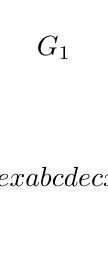
\begin{tikzpicture}
[scale =.35]
\GraphInit[vstyle=Welsh]
\SetGraphUnit{1.6}
%\SetVertexNoLabel
\node at (4,5) {$G_1$};
\node at (4,-2) {}; % To raise graph to match G2
\Vertex[LabelOut,Lpos=90,x=0,y=2]{$a$}
\Vertex[LabelOut,Lpos= 90,x=2,y=2]{$b$}
\Vertex[LabelOut,Lpos= 90,x=4,y=2]{$c$}
\Vertex[LabelOut,Lpos= 90,x=6,y=2]{$d$}
\Vertex[LabelOut,Lpos= 90,x=8,y=2]{$e$}
\Vertex[LabelOut,Lpos= 0,x=4,y=0]{$x$}
\Edges($a$, $b$, $c$, $d$, $e$)
\Edges($c$,$x$)
\end{tikzpicture}
\hspace{1in} %%
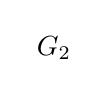
\begin{tikzpicture}
[scale =.35]
\GraphInit[vstyle=Welsh]
\SetGraphUnit{1.6}
%\SetVertexNoLabel
\node at (4,5) {$G_2$};
\Vertex[LabelOut,Lpos=90,x=0,y=2]{$a$}
\Vertex[LabelOut,Lpos= 90,x=2,y=2]{$b$}
\Vertex[LabelOut,Lpos= 90,x=4,y=2]{$c$}
\Vertex[LabelOut,Lpos= 0,x=4,y=0]{$d$}
\Vertex[LabelOut,Lpos= 0,x=4,y=-2]{$e$}
\Vertex[LabelOut,Lpos= 90,x=6,y=2]{$x$}
\Edges($a$, $b$, $c$, $d$, $e$)
\Edges($c$,$x$)
\end{tikzpicture}

                \caption{Isomorphic graphs}
                \label{fig_G1G2_labeled}
            \end{figure}      
        \item A \vocab{planarity-style move} on a graph drawing consists of moving one vertex $v$ to a different location and redrawing the edges from $v$ in its new location to each of $v$'s neighbors. \footnote{These moves are named for the game ``Planarity'' from \Cref{act_planarity_puzzle}.} 
    \end{apart}
\end{defn}

These moves give us another way to work with graph isomorphism.

\begin{rem}[Planarity-style moves]
\label{rem_planarity_moves}
    Graphs $G$ and $H$ are isomorphic exactly when we can transform a graph drawing of $G$ into a graph drawing of $H$ using a sequence of planarity-style moves. While visualizing such a transformation is a useful way to \emph{decide} if two graphs are isomorphic, to \emph{prove} that two graphs are isomorphic, you need to label the vertices according to the definition.  If you can see the transformation, just follow the vertices to see what the labels should be. For example, we can think of transforming the graph $G_1$ into the graph $G_2$ from \Cref{defn_ism_graphs} by shifting the vertex $x$ up and to the right and the vertices $d$ and $e$ down and to the left.
\end{rem}
 
When two graphs are complicated, it can be useful to compare their complements instead.  Note that if $G$ and $H$ are isomorphic and labeled with the same vertices and edges, then that labeling shows that $\overline{G}$ and $\overline{H}$ have the same vertices and edges and so $\overline{G}$ and $\overline{G}$ are also isomorphic.  We have the following result.

\begin{thm}[Isomorphic Complements]
\label{thm_ism_complement}
    For graphs $G$ and $H$ we have $G \cong H$ exactly when $\overline{G} \cong \overline{H}$.
\end{thm}

Here is an example of using the complement to prove that two graphs are isomorphic.

\begin{exam}[Using complements to prove isomorphic graphs]
\label{exam_prove_ism_complements}
    Consider the graphs $G$ and $H$ drawn in \Cref{fig_ism_Ham6}. 
        \begin{figure}[hbtp]
            \centering
            %Used in \Cref{sec_graph_ism}

\begin{tikzpicture}
[scale =.5, auto=left]
\GraphInit[vstyle=Welsh]
\SetGraphUnit{1.6}
\SetVertexNoLabel
\node at (0,3) {$G$};
\Vertices{circle}{$c$,$b$,$a$,$f$,$e$,$d$}
\Edges($a$,$b$,$c$,$d$,$e$,$f$,$a$)
\Edges($b$,$f$,$c$,$e$,$b$)
\Edges($a$,$e$)
\end{tikzpicture}
\hspace{1in}%%%%%
\begin{tikzpicture}
[scale =.5, auto=left]
\GraphInit[vstyle=Welsh]
\SetGraphUnit{1.6}
\SetVertexNoLabel
\node at (0,3) {$H$};
\Vertices{circle}{$e$,$a$,$b$,$f$,$c$,$d$}
\Edges($a$,$b$,$c$,$d$,$e$,$f$,$a$)
\Edges($b$,$f$,$c$,$e$,$b$)
\Edges($a$,$e$)
\end{tikzpicture}
            \caption{Are the graphs $G$ and $H$ isomorphic?}
            \label{fig_ism_Ham6}
        \end{figure}
        \begin{apart}
            \item Draw their complements.
                \begin{soln}
                    The complements $\overline{G}$ and $\overline{H}$ are drawn in \Cref{fig_ism_Ham6_comp}.
                    \begin{figure}[hbtp]
                        \centering
                        %Used in \Cref{sec_graph_ism}

\begin{tikzpicture}
[scale =.5, auto=left]
\GraphInit[vstyle=Welsh]
\SetGraphUnit{1.6}
\SetVertexNoLabel
\node at (0,2.5) {$\overline{G}$};
\Vertices{circle}{$c$,$b$,$a$,$f$,$e$,$d$}
\Edges($f$,$d$,$a$,$c$)
\Edges($b$,$d$)
\end{tikzpicture}
\hspace{1in}%%%%%
\begin{tikzpicture}
[scale =.5, auto=left]
\GraphInit[vstyle=Welsh]
\SetGraphUnit{1.6}
\SetVertexNoLabel
\node at (0,2.5) {$\overline{H}$};
\Vertices{circle}{$e$,$a$,$b$,$f$,$c$,$d$}
\Edges($f$,$d$,$a$,$c$)
\Edges($b$,$d$)
\end{tikzpicture}
                        \caption{Complements of graphs from \Cref{fig_ism_Ham6}.}
                        \label{fig_ism_Ham6_comp}
                    \end{figure}
                \end{soln}
            \item Label the vertices of the complements to show  $\overline{G} \cong \overline{H}$.
                \begin{soln}
                    We label the isolated vertex $z$, the degree 3 vertex $a$, and the degree 2 vertex $b$.  There is one leaf adjacent to $b$ which we label $c$.  Last, we label the other two leaves $u$ and $v$ (in either order). \Cref{fig_ism_Ham6_comp_labeled} shows these complements labeled as well as a simplified graph drawing of the complement.
                        \begin{figure}[hbtp]
                            \centering
                            %Used in \Cref{sec_graph_ism}

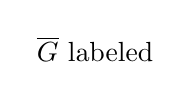
\begin{tikzpicture}
[scale =.5, auto=left]
\GraphInit[vstyle=Welsh]
\SetGraphUnit{1.6}
%\SetVertexNoLabel
\node at (0,4) {$\overline{G}$ labeled};
\Vertices{circle}{$c$,$u$,$b$,$v$,$z$,$a$}
\Edges($v$,$a$,$b$,$c$)
\Edges($u$,$a$)
\end{tikzpicture}
\hspace{.5in} %%%%%%%%%
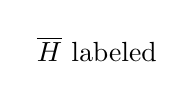
\begin{tikzpicture}
[scale =.5, auto=left]
\GraphInit[vstyle=Welsh]
\SetGraphUnit{1.6}
%\SetVertexNoLabel
\node at (0,4) {$\overline{H}$ labeled};
\Vertices{circle}{$z$,$b$,$u$,$v$,$c$,$a$}
\Edges($v$,$a$,$b$,$c$)
\Edges($u$,$a$)
\end{tikzpicture}
\hspace{.5in} %%%%%%%%%%%
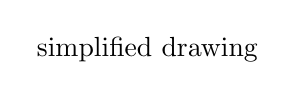
\begin{tikzpicture}
[scale =.5, auto=left]
\GraphInit[vstyle=Welsh]
\SetGraphUnit{1.6}
%\SetVertexNoLabel
\node at (6,4) {simplified drawing};
\Vertex[LabelOut,Lpos=-90,x=6,y=2]{$c$}
\Vertex[LabelOut,Lpos=-90,x=4,y=2]{$b$}
\Vertex[LabelOut,Lpos=-90,x=2,y=2]{$a$}
\Vertex[LabelOut,Lpos=90,x=0,y=3]{$u$}
\Vertex[LabelOut,Lpos=-90,x=0,y=1]{$v$}
\Vertex[LabelOut,Lpos=-90,x=8,y=2]{$z$}
\Edges($v$,$a$,$b$,$c$)
\Edges($u$,$a$)
\end{tikzpicture}
                            \caption{Labeling the complements from \Cref{fig_ism_Ham6_comp}.}
                            \label{fig_ism_Ham6_comp_labeled}
                        \end{figure}
                \end{soln}
            \item Is $G \cong H$? Explain.
                \begin{soln}
                    Yes, by \Cref{thm_ism_complement} since $\overline{G} \cong \overline{H}$, it follows that $G \cong H$.
                \end{soln}
        \end{apart}
\end{exam}

Practice showing graphs are isomorphic.

\begin{act}[Show two graphs are isomorphic]
\label{act_show_isomorphic}
~
    \begin{actpart}
        \item \label{part_ism_act_trees} Show the trees drawn in \Cref{fig_ism_trees} are isomorphic by labeling the vertices of each and listing the edges. Choose your labeling carefully.
            \begin{figure}[hbtp]
                \centering
                %Used in \Cref{sec_graph_ism}.

\begin{tikzpicture}
[scale =.35]
\GraphInit[vstyle=Welsh]
\SetGraphUnit{1.6}
\SetVertexNoLabel
%\node at (-2,4) {$T_1$};
\Vertex[LabelOut,Lpos=90,x=0,y=0]{$a$}
\Vertex[LabelOut,Lpos= 90,x=2,y=0]{$b$}
\Vertex[LabelOut,Lpos= 90,x=4,y=0]{$c$}
\Vertex[LabelOut,Lpos= 90,x=6,y=0]{$d$}
\Vertex[LabelOut,Lpos= 90,x=8,y=0]{$e$}
\Vertex[LabelOut,Lpos= 90,x=2,y=2]{$r$}
\Vertex[LabelOut,Lpos= 90,x=2,y=4]{$s$}
\Vertex[LabelOut,Lpos= 90,x=2,y=-2]{$y$}
\Vertex[LabelOut,Lpos= 90,x=2,y=-4]{$z$}
\Edges($a$, $b$, $c$, $d$, $e$)
\Edges($s$, $r$, $b$, $y$, $z$)
\end{tikzpicture}
\hspace{1 in} %%%%%
\begin{tikzpicture}
[scale =.35]
\GraphInit[vstyle=Welsh]
\SetGraphUnit{1.6}
\SetVertexNoLabel
%\node at (2,4) {$T_2$};
\node at (0,-4) {}; % to raise T2
\Vertex[LabelOut,Lpos=90,x=0,y=0]{$a$}
\Vertex[LabelOut,Lpos= 90,x=2,y=0]{$b$}
\Vertex[LabelOut,Lpos= 90,x=4,y=0]{$c$}
\Vertex[LabelOut,Lpos= 90,x=6,y=0]{$d$}
\Vertex[LabelOut,Lpos= 90,x=8,y=0]{$e$}
\Vertex[LabelOut,Lpos= 90,x=10,y=0]{$f$}
\Vertex[LabelOut,Lpos= 90,x=6,y=2]{$r$}
\Vertex[LabelOut,Lpos= 90,x=6,y=4]{$s$}
\Vertex[LabelOut,Lpos= 90,x=6,y=-2]{$y$}
\Edges($a$, $b$, $c$, $d$, $e$,$f$)
\Edges($s$, $r$, $d$, $y$)
\end{tikzpicture}
                \caption{Isomorphic trees for \Cref{act_show_isomorphic} (\ref{part_ism_act_trees}).}
                \label{fig_ism_trees}
            \end{figure}        
        \item \label{part_ism_act_Ham6} Show the two graphs drawn in \Cref{fig_ism_notK33} are isomorphic by labeling the vertices of each and listing the edges. Choose your labeling carefully.
            \begin{figure}[hbtp]
                \centering
                %Used in \Cref{sec_graph_ism}.

\begin{tikzpicture}
[scale =.25]
\GraphInit[vstyle=Welsh]
\SetGraphUnit{1.6}
\SetVertexNoLabel
%\node at (-2,8) {$S_1$};
\Vertex[LabelOut,Lpos=90,x=0,y=2]{$a$}
\Vertex[LabelOut,Lpos= 90,x=0,y=5]{$b$}
\Vertex[LabelOut,Lpos= 90,x=3,y=7]{$c$}
\Vertex[LabelOut,Lpos= 90,x=6,y=5]{$d$}
\Vertex[LabelOut,Lpos= 90,x=6,y=2]{$e$}
\Vertex[LabelOut,Lpos= 90,x=3,y=0]{$r$}
\Edges($a$, $b$, $c$, $d$, $e$,$r$,$a$)
\Edges($c$,$r$)
\Edges($b$,$d$)
\Edges($a$,$e$)
\end{tikzpicture}
\hspace{1in} %%%%%
\begin{tikzpicture}
[scale =.25]
\GraphInit[vstyle=Welsh]
\SetGraphUnit{1.6}
\SetVertexNoLabel
%\node at (-2,8) {$S_2$};
\Vertex[LabelOut,Lpos=90,x=0,y=0]{$a$}
\Vertex[LabelOut,Lpos= 90,x=0,y=6]{$e$}
\Vertex[LabelOut,Lpos= 90,x=4.25,y=3]{$c$}
\Vertex[LabelOut,Lpos= 90,x=6,y=6]{$d$}
\Vertex[LabelOut,Lpos= 90,x=6,y=0]{$b$}
\Vertex[LabelOut,Lpos= 90,x=1.75,y=3]{$r$}
\Edges($a$, $b$, $c$, $d$, $e$,$r$,$a$)
\Edges($c$,$r$)
\Edges($b$,$d$)
\Edges($a$,$e$)
\end{tikzpicture}
                \caption{Isomorphic graphs for \Cref{act_show_isomorphic} (\ref{part_ism_act_Ham6}).}
                \label{fig_ism_notK33}
            \end{figure}
        \item \label{part_ism_act_comp} Show that the graphs drawn in \Cref{fig_act_ism_comp} are isomorphic by showing their complements are isomorphic.  Label the complements and list the edges.
            \begin{figure}[hbtp]
                \centering
                %Used in \Cref{sec_graph_ism}.

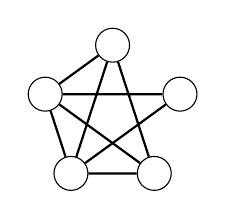
\begin{tikzpicture}
%[scale=1.2,auto=left,every node/.style={circle,fill=black}]
[scale=0.9,auto=left,every node/.style={circle,draw=black, fill=white, inner sep=.06in}]
\node (1) at (90+0*72:1) {};
\node  (2) at (90+1*72:1) {};
\node  (3) at (90+2*72:1) {};
\node  (4) at (90+3*72:1) {};
\node  (5) at (90+4*72:1) {};
%\node  (0) at (90+4*72:0) {0};
%\node  (0) at (0 ,0) {0};
\draw [thick] (1) to (2) to (3) to (4);
\draw [thick] (1) to (3) to (5) to (2) to (4) to (1);
\end{tikzpicture}
\hspace{1in} %%%%%
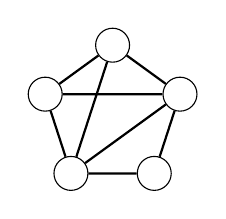
\begin{tikzpicture}
[scale=0.9,auto=left,every node/.style={circle,draw=black, fill=white, inner sep=.06in}]
\node (1) at (90+0*72:1) {};
\node  (2) at (90+1*72:1) {};
\node  (3) at (90+2*72:1) {};
\node  (4) at (90+3*72:1) {};
\node  (5) at (90+4*72:1) {};
%\node  (0) at (90+4*72:0) {0};
%\node  (0) at (0 ,0) {0};
\draw [thick] (1) to (2) to (3) to (4) to (5) to (1);
\draw [thick] (1) to (3) to (5) to (2);
\end{tikzpicture}
                \caption{Isomorphic graphs for \Cref{act_show_isomorphic} (\ref{part_ism_act_comp}).}
                \label{fig_act_ism_comp}
            \end{figure}
        \item \label{part_petersen} Show that the graphs drawn in \Cref{fig_ism_petersen} are isomorphic by labeling the vertices so they have the same edges.  Hint: start with a 6-cycle in the graph on the left.
            \begin{figure}[hbtp]
                \centering
                %Used in \Cref{sec_graph_ism}.

\begin{tikzpicture}
[scale =.35]
\GraphInit[vstyle=Welsh]
\SetGraphUnit{1.6}
\SetVertexNoLabel
% Inner circle
\Vertex[LabelOut,Lpos=112,x=0.618,y=1.90]{$a$}
\Vertex[LabelOut,Lpos=40,x=2,y=0]{$b$}
\Vertex[LabelOut,Lpos= -32,x=0.618,y=-1.90]{$c$}
\Vertex[LabelOut,Lpos= -104,x=-1.61,y=-1.17]{$d$}
\Vertex[LabelOut,Lpos= 184,x=-1.61,y=1.17]{$e$}
\Edges($a$,$c$,$e$,$b$,$d$,$a$)
% Outer circle
\Vertex[LabelOut,Lpos=112,x=1.30,y=3.99]{$A$}
\Vertex[LabelOut,Lpos=40,x=4.2,y=0]{$B$}
\Vertex[LabelOut,Lpos= -32,x=1.30,y=-3.99]{$C$}
\Vertex[LabelOut,Lpos= -104,x=-3.38,y=-2.46]{$D$}
\Vertex[LabelOut,Lpos= 184,x=-3.38,y=2.46]{$E$}
\Edges($A$,$B$,$C$,$D$,$E$,$A$)
% Spokes
\Edges($a$,$A$)
\Edges($b$,$B$)
\Edges($c$,$C$)
\Edges($d$,$D$)
\Edges($e$,$E$)
\end{tikzpicture}
\hspace{1 in} %%%%%
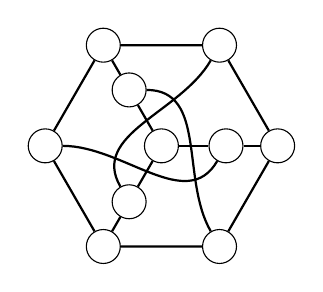
\begin{tikzpicture}
[scale=.82,auto=left,every node/.style={circle,draw=black, fill=white, inner sep=.06in}]
\node (1) at (1*60:1.8) {};
\node (2) at (2*60:1.8) {};
\node (3) at (3*60:1.8) {};
\node (4) at (4*60:1.8) {};
\node (5) at (5*60:1.8) {};
\node (6) at (6*60:1.8) {};
\node(7) at (1*120:1) {};
\node(8) at (2*120:1) {};
\node(9) at (3*120:1) {};
\node(10) at (1*0:0) {};  
\draw[thick] (1) to (2) to (3) to (4) to (5) to (6) to (1);
\draw[thick] (2) to (7) to (10);
\draw[thick] (6) to (9) to (10);
\draw[thick] (4) to (8) to (10);
\draw[thick] (1) to [out=240, in=120,looseness=1](8) ;
\draw[thick] (5) to [out=120, in=0,looseness=1](7) ;
\draw[thick] (3) to [out=0, in=240,looseness=1](9) ;
\end{tikzpicture}
                \caption{Two drawings of the Petersen graph for \Cref{act_show_isomorphic} (\ref{part_petersen}) and \Cref{exer_petersen}.}
                \label{fig_ism_petersen}
            \end{figure}
    \end{actpart}
\end{act}

%%%%%%%%%%%%%%%%%%%%%%%%%%%%%%%%%%%%%%%%%%

\newcommand{\subgraphtrees}{Subgraphs and Trees}
\subsection{\subgraphtrees}
\label{sub_subgraph_tree}

A common type of graph used to store information in a computer is a \vocab{tree}. We saw examples of possibility trees in \Cref{sec_listing}.  Trees are defined using the concepts of subgraph and connectivity, so we start there.

\begin{defn}[Subgraph]
\label{defn_subgraph}
    The graph $H$ is a \vocab{subgraph} of the graph $G$ if each vertex of $H$ is a vertex of $G$ and each edge of $H$ is an edge of $G$. Note that since $H$ is a graph, each edge of $H$ necessarily contains two vertices of $H$. For example, in \Cref{fig_subgraph_order6}, the graph on the left is a subgraph of the graph on the right.
        \begin{figure}[hbtp]
            \centering
            %Used in \Cref{sec_subgraph_isomorphic}.


% Subgraph H
\begin{tikzpicture}
[scale =.5]
\GraphInit[vstyle=Welsh]
\SetGraphUnit{1.6}
%\SetVertexNoLabel
\node at (1,5.5) {$H$};
\Vertex[LabelOut,Lpos=135,x=0,y=3.5]{$a$} 
\Vertex[LabelOut,Lpos=45,x=1.6,y=3.5]{$b$}
\Vertex[LabelOut,Lpos=-135,x=0,y=1]{$e$} 
\Vertex[LabelOut,Lpos=-45,x=1.6,y=1]{$d$} 
\Edges($e$,$b$,$d$,$e$,$a$)
\end{tikzpicture}
%%%%%%%%%%%%%%%%%%%%%%%
\hspace{1in} %%%%%%%%%%
%%%%%%%%%%%%%%%%%%%%%%%
% G
\begin{tikzpicture}
[scale =.5]
\GraphInit[vstyle=Welsh]
\SetGraphUnit{1.6}
%\SetVertexNoLabel
\node at (0,3) {$G$};
\Vertices{circle}{$c$,$b$, $a$, $f$,$e$, $d$}
\Edges($a$, $b$, $c$, $d$, $e$,$a$)
\Edges($c$,$f$)
\Edges($e$,$b$,$d$)
\end{tikzpicture}

            \caption{The graph $H$ is a subgraph of the graph $G$.}
            \label{fig_subgraph_order6}
        \end{figure} 
\end{defn}

In \Cref{fig_subgraph_order6}, we draw the vertices of the subgraph $H$ in the same position as they appeared in $G$, but that is not required.

\begin{exam}[Less obvious subgraphs]
\label{exam_less_obvious_subgraphs}
    Consider the graph $G$ from \Cref{fig_subgraph_order6}.  Which of the following graphs are subgraphs of $G$?
        \begin{apart}
            \item \label{part_cycle_subgraph} The cycle $C$ drawn in \Cref{fig_less_obv_cycle}.
                \begin{figure}[hbtp]
                    \centering
                    %Used in \Cref{sec_graph_thy}.

\begin{tikzpicture}
[scale =.35]
\GraphInit[vstyle=Welsh]
\SetGraphUnit{1.6}
%\SetVertexNoLabel
\Vertex[LabelOut,Lpos=180,x=0,y=4]{$b$}
\Vertex[LabelOut,Lpos= 0,x=4,y=4]{$c$}
\Vertex[LabelOut,Lpos= 0,x=4,y=0]{$d$}
\Vertex[LabelOut,Lpos= 180,x=0,y=0]{$e$}
\Edges($b$, $c$, $d$, $e$, $b$)
\end{tikzpicture}
                    \caption{The graph $C$ from \Cref{exam_less_obvious_subgraphs}.}
                    \label{fig_less_obv_cycle}
                \end{figure}
                \begin{soln}
                    The cycle $C$ is a subgraph of $G$ because each of $C$'s vertices ($b$, $c$, $d$, and $e$) and each of $C$'s edges ($\{b,c\}$, $\{c,d\}$, $\{d,e\}$, and $\{e,b\}$) are in $G$.  Note that $C$ is the cycle $C_4$, so we say $C_4$ is a subgraph of $G$.
                    \end{soln}

            \item \label{part_path_subgraph}The path $P$ drawn in \Cref{fig_less_obv_path}.
                \begin{figure}[hbtp]
                    \centering
                    %Used in \Cref{sec_graph_thy}.

\begin{tikzpicture}
[scale =.35]
\GraphInit[vstyle=Welsh]
\SetGraphUnit{1.6}
%\SetVertexNoLabel
\Vertex[LabelOut,Lpos=-90,x=0,y=0]{$f$}
\Vertex[LabelOut,Lpos=-90,x=3,y=0]{$c$}
\Vertex[LabelOut,Lpos= -90,x=6,y=0]{$b$}
\Vertex[LabelOut,Lpos= -90,x=9,y=0]{$e$}
\Vertex[LabelOut,Lpos= -90,x=12,y=0]{$a$}
\Edges($f$, $c$, $b$, $e$, $a$)
\end{tikzpicture}
                    \caption{The graph $P$ from \Cref{exam_less_obvious_subgraphs}.}
                    \label{fig_less_obv_path}
                \end{figure}
                \begin{soln}
                    The path $P$ is a subgraph of $F$ because each of $P$'s vertices ($a$, $c$, $d$, $e$, and $f$) and each of $P$'s edges (\{f,c\}, \{c,b\}, \{b,e\}, and \{e,a\}) are in $F$. Note that $P$ is the path $P_5$, so we say $P_5$ is a subgraph of $G$.
                    \end{soln}

            \item The graph $J$ drawn in \Cref{fig_less_obv_clique}.
                \begin{figure}[hbtp]
                    \centering
                    %Used in \Cref{sec_graph_thy}.

\begin{tikzpicture}
[scale =.35]
\GraphInit[vstyle=Welsh]
\SetGraphUnit{1.6}
%\SetVertexNoLabel
\Vertex[LabelOut,Lpos=180,x=0,y=4]{$a$}
\Vertex[LabelOut,Lpos= 0,x=4,y=4]{$b$}
\Vertex[LabelOut,Lpos= 0,x=4,y=0]{$d$}
\Vertex[LabelOut,Lpos= 180,x=0,y=0]{$e$}
\Edges($a$, $b$, $d$, $e$, $b$,$a$)
\Edges($a$,$d$)
\Edges($b$,$e$)
\end{tikzpicture}
                    \caption{The graph $J$ from \Cref{exam_less_obvious_subgraphs}.}
                    \label{fig_less_obv_clique}
                \end{figure}
                \begin{soln}
                    The graph $J$ is not a subgraph of $G$ because $\{a,d\}$ is an edge in $J$ but not in $G$.
                \end{soln}
                    
            \item The graph $D$ drawn in \Cref{fig_less_obv_subgraph}.
                \begin{figure}[hbtp]
                    \centering
                    %Used in \Cref{sec_graph_thy}.

\begin{tikzpicture}
[scale =.35]
\GraphInit[vstyle=Welsh]
\SetGraphUnit{1.6}
%\SetVertexNoLabel
%%% Cycle
\Vertex[LabelOut,Lpos=180,x=0,y=4]{$a$}
\Vertex[LabelOut,Lpos= 0,x=4,y=4]{$b$}
\Vertex[LabelOut,Lpos= 0,x=4,y=0]{$d$}
\Vertex[LabelOut,Lpos= 180,x=0,y=0]{$e$}
\Edges($a$, $e$)
\Edges($b$,$e$,$d$)
%%% Path
\Vertex[LabelOut,Lpos= -90,x=8,y=2]{$c$}
\Vertex[LabelOut,Lpos= -90,x=12,y=2]{$f$}
\Edges($c$,$f$)

\end{tikzpicture}
                    \caption{The graph $D$ from \Cref{exam_less_obvious_subgraphs}.}
                    \label{fig_less_obv_subgraph}
                \end{figure}
                \begin{soln}
                    The graph $D$ is a subgraph of $F$ since each vertex and edge in $D$ is in $G$, even though $D$ has two separate pieces.
                \end{soln}
        \end{apart}
\end{exam}

We introduce a bit more vocabulary about subgraphs.

\begin{defn}[Cyclic subgraphs]
\label{defn_cyclic_subgraphs}
~
    \begin{apart}
        \item A \vocab{cyclic subgraph} of a graph is a subgraph that is a copy of $C_s$ for some integer $s \ge 3$.  For example, the graph $C$ from \Cref{exam_less_obvious_subgraphs} was a cyclic subgraph of the graph $G$.  
        \item A graph $G$ \vocab{contains an $s$ cycle} if $C_s$ is a subgraph for some $s \ge 3$.  For example, the graph $G$ in \Cref{fig_subgraph_order6} contains several 3-cycles, a couple of 4-cycles, and 5-cycle.   
        \item A graph is \vocab{acyclic} if it does not contain any cyclic subgraphs. For example, the path graphs $P_s$ are acyclic.
    \end{apart}  
\end{defn}

Let's count all the cycles in a graph.

\begin{exam}[Counting cycles]
\label{exam_count_cycles}
    Count all the cycles in the graph $G$ in \Cref{fig_subgraph_order6}.
        \begin{soln}
            First, there are three 3-cycles: one with vertices $a$, $b$, and $e$; a second with vertices $b$, $d$, and $e$; and a third with vertices $b$, $c$, and $d$.

            Next, there are two 4-cycles: one with vertices $a$, $b$, $d$, and $e$ and the other with vertices $b$, $c$, $d$, and $e$.

            Lastly, there is one 5-cycle with vertices $a$, $b$, $c$, $d$, and $e$.
            %SU could have drawing of all these subgraphs (or not)
        \end{soln}
\end{exam}

In most networks, we want to maintain connectivity.  Casually speaking, a graph is connected if there are no separate pieces, which is difficult to define directly.  We give a formal definition of connected here.

\begin{defn}[Paths and connectivity]
\label{defn_path_connected}
~
    \begin{apart}
        \item A \vocab{path} in a graph is a subgraph that is a copy of $P_s$ for some integer $s \ge 1$.  For example, the graph $P$ from \Cref{exam_less_obvious_subgraphs} was a path in the graph $G$. 
        
        \item A \vocab{$uv$-path} is a path with endpoints $u$ and $v$.  For example, the graph $P$ from \Cref{exam_less_obvious_subgraphs} is a $fa$-path (or an $af$-path) in the graph $G$. 
        A single vertex $u$ is considered a $uu$-path. 
        
        \item A graph $G$ is \vocab{connected} if for all vertices $u$, $v$ there exists a $uv$-path in $G$.  For example, the graph $G$ in \Cref{fig_subgraph_order6} is connected, as are its subgraphs $C$ and $P$ from \Cref{exam_less_obvious_subgraphs}.

        \item A graph $G$ that is not connected is \vocab{disconnected}.  For example, the subgraph $D$ in \Cref{exam_less_obvious_subgraphs} was disconnected because, for example, there does not exist a $cd$-path in $D$.
    \end{apart}
\end{defn}

Let's look at an example.

\begin{exam}[Finding paths]
\label{exam_finding paths}
    Consider the graph $G$ drawn in \Cref{fig_house_with_tails}.  
    Find an $hd$-path in $G$.  Is it unique?
        \begin{soln}
            One $hd$-path is $hcd$.  It is not unique.  For example $hjibcd$ is another $hd$-path as is $hibcd$.
        \end{soln}
\end{exam}

        \begin{figure}[hbtp]
            \centering
            %Used in \Cref{sec_graph_thy}
% House with tails

\begin{tikzpicture}
    [scale =.35]
    \GraphInit[vstyle=Welsh]
    \SetGraphUnit{1.6}
        %\SetVertexNoLabel
    % bottom row
    \Vertex[LabelOut,Lpos=-90,x=0,y=0]{$a$}
    \Vertex[LabelOut,Lpos=-90,x=3,y=0]{$b$} 
    \Vertex[LabelOut,Lpos=-90,x=6,y=0]{$c$}
    \Vertex[LabelOut,Lpos=-90,x=9,y=0]{$d$}    
    \Vertex[LabelOut,Lpos=-90,x=12,y=0]{$e$}
    \Edges($a$,$b$,$c$,$d$,$e$)
    % top row and roof peak
    \Vertex[LabelOut,Lpos=90,x=4.5,y=5]{$j$}
    \Vertex[LabelOut,Lpos=135,x=3,y=3]{$i$} 
    \Vertex[LabelOut,Lpos=45,x=6,y=3]{$h$}
    \Vertex[LabelOut,Lpos=90,x=9,y=3]{$g$}    
    \Vertex[LabelOut,Lpos=90,x=12,y=3]{$f$}
    % tails
    \Edges($f$,$g$,$c$)
    \Edges($h$,$i$,$j$,$h$)
    % vertical edges
    \Edges($b$,$i$)
    \Edges($c$,$h$)
\end{tikzpicture}
            \caption{The graph $G$ from \Cref{exam_finding paths}.}
            \label{fig_house_with_tails}
        \end{figure}

We can now define a tree.  Many applications of graph theory in computer science use trees.

\begin{defn}[Tree]
\label{defn_tree}
    A \vocab{tree} is an connected acyclic graph.  For example, the path graphs $P_s$ are trees for $s \ge 1$.  The graph $T$ drawn in \Cref{fig_tree_defn} is also a tree.

    \begin{figure}[hbtp]
        \centering
        %Used in \Cref{sec_graph_thy} and again in 
%\Cref{sec_fn_words}

\begin{tikzpicture}
[scale =.35]
\GraphInit[vstyle=Welsh]
\SetGraphUnit{1.6}
%\SetVertexNoLabel
\Vertex[LabelOut,Lpos= 90,x=0,y=9]{$n$}
\Vertex[LabelOut,Lpos= 90,x=3,y=9]{$p$}
\Vertex[LabelOut,Lpos= 90,x=6,y=9]{$q$}
\Vertex[LabelOut,Lpos= -90,x=0,y=6]{$r$}
\Vertex[LabelOut,Lpos= -90,x=3,y=6]{$s$}
\Vertex[LabelOut,Lpos= 90,x=6,y=6]{$t$}
\Vertex[LabelOut,Lpos= 90,x=9,y=6]{$u$}
\Vertex[LabelOut,Lpos= 90,x=12,y=6]{$v$}
\Vertex[LabelOut,Lpos= 180,x=6,y=3]{$w$}
\Vertex[LabelOut,Lpos= -90,x=9,y=3]{$x$}
\Vertex[LabelOut,Lpos= 180,x=6,y=0]{$y$}
\Vertex[LabelOut,Lpos= 180,x=6,y=-3]{$z$}
\Edges($r$, $s$, $w$, $y$, $z$)
\Edges($y$,$x$,$v$)
\Edges($n$,$s$,$p$)
\Edges($x$,$u$,$q$)
\Edges($w$,$t$)
\end{tikzpicture}
        \caption{An example of a tree $T$.}
        \label{fig_tree_defn}
    \end{figure}
\end{defn}

A tree needs to be connected and acyclic.  If either condition fails in a graph, then that graph is not a tree.

\begin{exam}[Not a tree]
\label{exam_not_a_tree}
    Explain why each graph is not a tree.
        \begin{apart}
            \item The graph $G$ drawn in \Cref{fig_house_with_tails}.
                \begin{soln}
                    The graph $G$ is connected, but it is not a tree because it is not acyclic.  For example, $G$ contains a 3-cycle with vertices $i$, $j$, and $h$.  By the way, $G$ also contains a 4-cycle with vertices $b$, $c$, $h$, and $i$ and a 5-cycle with vertices $b$, $c$, $h$, $i$, and $j$.
                \end{soln}
            \item The graph $D$ drawn in \Cref{fig_less_obv_subgraph}.
                \begin{soln}
                    The graph $D$ is acyclic, but it is not a tree because it is disconnected.  
                \end{soln}
        \end{apart}
\end{exam}

Try working with subgraphs and trees.

\begin{act}[Subgraphs and trees]
\label{act_subgraphs_trees}
    Consider the graphs $G$, $H$, and $K$ drawn in \Cref{fig_subgraphs_trees}.
        \begin{figure}[hbtp] 
            \centering
            %Used in \Cref{sec_graph_thy}.

%% G
\begin{tikzpicture}
    [scale =.35]
    \GraphInit[vstyle=Welsh]
    \SetGraphUnit{1.6}
    %\SetVertexNoLabel
    \node at (3,6) {$G$};
    % bottom row
    \Vertex[LabelOut,Lpos=-90,x=0,y=0]{$x$}
    \Vertex[LabelOut,Lpos=-90,x=3,y=0]{$y$} 
    \Vertex[LabelOut,Lpos=-90,x=6,y=0]{$z$}
    \Edges($x$,$y$,$z$)
    % top row
    \Vertex[LabelOut,Lpos=90,x=0,y=3]{$a$}
    \Vertex[LabelOut,Lpos=90,x=3,y=3]{$b$} 
    \Vertex[LabelOut,Lpos=90,x=6,y=3]{$c$}
    \Edges($a$,$b$,$c$)
    % vertical edges
    \Edges($b$,$y$)
    \Edges($c$,$z$)
    % the rest of the Xs
    \Edges($a$,$y$)
    \Edges($x$,$b$,$z$)
\end{tikzpicture}
%%
\hspace{.5in} %%%%%
%%
%% H
\begin{tikzpicture}
    [scale =.35]
    \GraphInit[vstyle=Welsh]
    \SetGraphUnit{1.6}
    %\SetVertexNoLabel
        \node at (3,6) {$H$};
    % new top row
    \Vertex[LabelOut,Lpos=-90,x=3,y=0]{$x$}
    % next layer
    \Vertex[LabelOut,Lpos= 90,x=0,y=3]{$b$} 
    \Vertex[LabelOut,Lpos= 90,x=6,y=3]{$y$} 
    % leaves  
    \Vertex[LabelOut,Lpos=-90,x=6,y=0]{$z$} 
    \Vertex[LabelOut,Lpos=-90,x=0,y=0]{$c$}
    % edges
    \Edges($x$,$y$,$z$)
    \Edges($b$,$c$)
    \Edges($b$,$y$)
    \Edges($x$,$b$)
\end{tikzpicture}
%%
\hspace{.5in} %%%%%
%%
%% K
\begin{tikzpicture}
    [scale =.35]
    \GraphInit[vstyle=Welsh]
    \SetGraphUnit{1.6}
    %\SetVertexNoLabel
        \node at (3,6) {$K$};
    % new top row
    \Vertex[LabelOut,Lpos=-90,x=4,y=0]{$a$}
    % next layer
    \Vertex[LabelOut,Lpos= 90,x=0,y=3]{$b$} 
    \Vertex[LabelOut,Lpos= 90,x=6,y=3]{$y$} 
    % leaves  
    \Vertex[LabelOut,Lpos=-90,x=8,y=0]{$c$} 
    \Vertex[LabelOut,Lpos=-90,x=0,y=0]{$z$}
    % edges
    \Edges($a$,$y$,$c$)
    \Edges($b$,$z$)
    \Edges($b$,$y$)
\end{tikzpicture}
            \caption{The graphs $G$, $H$, and $K$ from \Cref{act_subgraphs_trees}}
            \label{fig_subgraphs_trees}
        \end{figure}
        \begin{actpart}
            \item Confirm that $H$ is a subgraph of $G$.
            \item Explain why $K$ is not a subgraph of $G$.
            \item Find an $az$-path in $G$. Is it unique?  Explain.
            \item List the 3-cycles in $G$ by listing the three vertices in each 3-cycle.  Hint: There are four of them.
            \item List four 4-cycles in $G$ by listing the four vertices in each cycle in the order you would go around the cycle.  Hint: One looks like an X.
            \item How many 5-cycles does $G$ have?
            \item Check that $K$ is a tree.
            \item How are the number of vertices of $K$ and the number of edges of $K$ related?
        \end{actpart}
\end{act}

%%%%%%%%%%%%%%%%%%%%%%%%%%%%%%%%%%%%%%%%

\subsection{Exercises}

%%%%%%%%%%%%%%%%%%%%%%%%%%%%%%%%%%%%%%%%

\subsubsection*{Exercises for \Cref{sub_planarity}
\subplanarity}

\begin{exer}[\exerP] % Show complete bipartite graph $K_{2,t}$ is planar]
\label{exer_K2bn_planar}
   Explain how to draw the complete bipartite graph $K_{2,t}$ in the plane without edge crossings.
\end{exer}

\begin{exer}[\exerU] % Play planarity]
\label{exer_play_planarity}
    Play planarity at \url{https://www.jasondavies.com/planarity/}. Submit a screenshot of your solution to level eight of the puzzle in under two minutes.
\end{exer}

\begin{exer}[\exerR] % planariy
\label{exer_dyk_planarity}
    Do you know \ldots
        \begin{exerpart}
            \item What an edge crossing is?
            \item What a planar graph is?
        \end{exerpart}
\end{exer}

\begin{exer}[\exerE] % Play planarity]
\label{exer_play_planarity_higher_level}
    Play planarity at \url{https://www.jasondavies.com/planarity/}. Submit a screenshot of your solution to Level 16 of the puzzle.
\end{exer}

%%%%%%%%%%%%%%%%%%%%%%%%

\subsubsection*{Exercises for \Cref{sub_isomorphic_graphs}
\subisograph}

\begin{exer}[\exerP] % Show trees isomorphic.]
\label{exer_show_tree_ism}
    Prove the trees drawn in \Cref{fig_ism_trees_easy} are isomorphic by labeling the vertices of each tree so that they have the same set of vertices and edges.  
        \begin{figure}[hbtp]
            \centering
            %Used in \Cref{sec_subgraph_isomorphic}.

\begin{tikzpicture}
[scale =.35]
\GraphInit[vstyle=Welsh]
\SetGraphUnit{1.6}
\SetVertexNoLabel
%\node at (-2,4) {$T_3$};
\Vertex[LabelOut,Lpos=90,x=0,y=0]{$a$}
\Vertex[LabelOut,Lpos= 90,x=2,y=0]{$b$}
\Vertex[LabelOut,Lpos= 90,x=4,y=0]{$c$}
\Vertex[LabelOut,Lpos= 90,x=6,y=0]{$d$}
\Vertex[LabelOut,Lpos= 90,x=2,y=-2]{$u$}
\Vertex[LabelOut,Lpos= 90,x=2,y=-4]{$v$}
\Vertex[LabelOut,Lpos= 90,x=4,y=2]{$w$}
\Vertex[LabelOut,Lpos= 90,x=7.5,y=1.4]{$y$}
\Vertex[LabelOut,Lpos= 90,x=7.5,y=-1.4]{$z$}
\Edges($a$, $b$, $c$, $d$)
\Edges($b$, $u$, $v$)
\Edges($c$, $w$)
\Edges($y$,$d$,$z$)
\end{tikzpicture}
\hspace{1 in} %%%%%
\begin{tikzpicture}
[scale =.35]
\GraphInit[vstyle=Welsh]
\SetGraphUnit{1.6}
\SetVertexNoLabel
%\node at (-2,4) {$T_4$};
\node at (0,-4) {}; % to raise T4
\Vertex[LabelOut,Lpos=90,x=0,y=0]{$z$}
\Vertex[LabelOut,Lpos= 90,x=2,y=0]{$d$}
\Vertex[LabelOut,Lpos= 90,x=4,y=0]{$c$}
\Vertex[LabelOut,Lpos= 90,x=6,y=0]{$b$}
\Vertex[LabelOut,Lpos= 90,x=8,y=0]{$u$}
\Vertex[LabelOut,Lpos= 90,x=10,y=0]{$v$}
%%
\Vertex[LabelOut,Lpos= 90,x=6,y=2]{$a$}
\Vertex[LabelOut,Lpos= 90,x=4,y=2]{$w$}
\Vertex[LabelOut,Lpos= 90,x=2,y=2]{$y$}
\Edges($a$, $b$, $c$, $d$)
\Edges($b$, $u$, $v$)
\Edges($c$, $w$)
\Edges($y$,$d$,$z$)
\end{tikzpicture}

            \caption{Isomorphic trees for  \Cref{exer_show_tree_ism}.}
            \label{fig_ism_trees_easy}
        \end{figure}
\end{exer}

\begin{exer}[\exerP] % Show graphs isomorphic.]
\label{exer_show_graph_ism}
    Prove the graphs drawn in \Cref{fig_ism_Ham5} are isomorphic by labeling the vertices of each graph so that they have the same set of vertices and edges. 
        \begin{figure}[hbtp]
            \centering
            %Used in \Cref{sec_graph_thy}.

\begin{tikzpicture}
[scale =.55, auto=left]
\GraphInit[vstyle=Welsh]
\SetGraphUnit{1.6}
\SetVertexNoLabel
%\node at (0,3) {$G_3$};
\Vertices{circle}{$y$,$z$,$v$,$w$,$x$}
\Edges( $y$,$z$,$v$,$w$,$x$,$y$)
\Edges($z$,$x$,$v$,$z$)
\Edges($y$,$w$)
\end{tikzpicture}
\hspace{1in} %%%%%
\begin{tikzpicture}
[scale =.55, auto=left]
\GraphInit[vstyle=Welsh]
\SetGraphUnit{1.6}
\SetVertexNoLabel
%\node at (0,3) {$G_4$};
\Vertices{circle}{$y$,$z$,$v$,$w$}
\Vertex[LabelOut,Lpos= 90,x=0,y=0]{$x$}
\Edges( $y$,$z$,$v$,$w$,$x$,$y$)
\Edges($z$,$x$,$v$,$z$)
\Edges($y$,$w$)
\end{tikzpicture}

            \caption{Isomorphic graphs for \Cref{exer_show_graph_ism}.}
            \label{fig_ism_Ham5}
        \end{figure}
\end{exer}

\begin{exer}[\exerP] % Show graphs isomorphic using complement.]
\label{exer_show_graph_ism_using_comp}
    Prove the graphs drawn in \Cref{fig_ism_H4b7} are isomorphic by showing that their complements are isomorphic.     
        \begin{figure}[hbtp]
            \centering
            %Used in \Cref{sec_subgraph_tree}.

\begin{tikzpicture}
[scale =.55, auto=left]
\GraphInit[vstyle=Welsh]
\SetGraphUnit{1.6}
\SetVertexNoLabel
\node at (0,3) {$A$};
\Vertices{circle}{$y$,$z$,$t$,$u$, $v$,$w$,$x$}
\Edges($t$,$u$,$v$,$w$,$x$,$y$,$z$,$t$)
\Edges($u$,$w$,$y$,$t$,$v$,$x$,$z$,$u$)
\end{tikzpicture}
\hspace{1in} %%%%%
\begin{tikzpicture}
[scale =.55, auto=left]
\GraphInit[vstyle=Welsh]
\SetGraphUnit{1.6}
\SetVertexNoLabel
\node at (0,3) {$B$};
\Vertices{circle}{$t$,$x$,$u$,$y$, $v$,$z$,$w$}
\Edges($t$,$u$,$v$,$w$,$x$,$y$,$z$,$t$)
\Edges($u$,$w$,$y$,$t$,$v$,$x$,$z$,$u$)
\end{tikzpicture}
            \caption{Isomorphic graphs for \Cref{exer_show_graph_ism_using_comp}.}
            \label{fig_ism_H4b7}
        \end{figure}
\end{exer}

\begin{exer}[\exerU] % Petersen graph]
\label{exer_petersen}
    Show that the graphs drawn in \Cref{fig_ism_petersen} are isomorphic by labeling the vertices so that they have the same edges. Hint: Start with a 6-cycle in the graph on the left.  Yes, this exercise repeats \Cref{act_show_isomorphic} (\ref{part_petersen}). 
\end{exer}

\begin{exer}[\exerR] % isomorphic graphs
\label{exer_dyk_ism_graphs}
    Do you know \ldots
        \begin{exerpart}
            \item What it means when we say that two graphs are isomorphic?
            \item How to show that two graphs are isomorphic (by labeling the vertices)?
            \item How to use complements to show that two graphs are isomorphic?
            \item How to use planarity-style moves to decide if two graphs are isomorphic?
        \end{exerpart}
\end{exer}

\begin{exer}[\exerE] % self-complementary graphs]
\label{exer_selfcomp_graph}
    A graph $G$ is \vocab{self-complementary} if it isomorphic to its complement.  That is, if $G \cong \overline{G}$. 
        \begin{apart}           
            \item Show that the path $P_4$ is self-complementary. 
            \item Show that the cycle $C_5$ is self-complementary.
        \end{apart}
\end{exer}

\begin{exer}[\exerE] % edges in self-complementary graphs]
\label{exer_edges_selfcomp_graphs}  
    We defined self-complementary in \Cref{exer_selfcomp_graph}.
        \begin{exerpart}
            \item If $G$ is a self-complementary graph with four vertices, how many edges must it have? Explain. Hint: How many edges does the complete graph $K_4$ have?
            \item If $G$ is a self-complementary graph with five vertices, how many edges must it have? Explain. Hint: How many edges does the complete graph $K_5$ have?
        \end{exerpart}
\end{exer}

%%%%%%%%%%%%%%%%%%%%%%%%

\subsubsection*{Exercises for \Cref{sub_subgraph_tree}
\subgraphtrees}

\begin{exer}[\exerP] % subgraphs]
\label{exer_subgraphs}
   Consider the graphs $A$, $B$, and $C$ drawn in \Cref{fig_C8_plus_edges}.
       \begin{figure}[hbtp]
           \centering
           %Used in \Cref{sec_graph_thy}.

%% A
\begin{tikzpicture}
[scale =.55, auto=left]
\GraphInit[vstyle=Welsh]
\SetGraphUnit{1.6}
%\SetVertexNoLabel
\Vertices{circle}{$c$,$b$,$a$,$h$,$g$,$f$,$e$,$d$}
\Edges($a$,$b$,$c$,$d$,$e$,$f$,$g$,$h$,$a$)
\Edges($a$,$d$)
\Edges($c$,$g$)
\Edges($a$,$f$)
\end{tikzpicture}
%%
\hspace{.5in}
%%
%% B
\begin{tikzpicture}
[scale =.55, auto=left]
\GraphInit[vstyle=Welsh]
\SetGraphUnit{1.6}
%\SetVertexNoLabel
\Vertices{circle}{$c$,$d$,$a$,$f$,$g$}
\Edges($a$,$f$,$g$,$c$,$d$,$a$)
\end{tikzpicture}
%%
\hspace{.5in}
%%
%% C
\begin{tikzpicture}
[scale =.55, auto=left]
\GraphInit[vstyle=Welsh]
\SetGraphUnit{1.6}
%\SetVertexNoLabel
\Vertices{circle}{$c$,$d$,$a$,$g$}
\Edges($a$,$g$,$c$,$d$,$a$)
\end{tikzpicture}


           \caption{From left-to-right, the graphs  $A$, $B$, and $C$. }
           \label{fig_C8_plus_edges}
       \end{figure}
        \begin{exerpart}
            \item Show how to check that $B$ is a subgraph of $A$.
            \item Explain why $C$ is not a subgraph of $A$.  
        \end{exerpart}
\end{exer}

\begin{exer}[\exerP] % cyclic subgraphs]
\label{exer_cyclic_subgraphs}
    Again, consider the graphs $A$, $B$, and $C$ drawn in \Cref{fig_C8_plus_edges}.
        \begin{exerpart}
            \item Draw a 4-cycle that is a subgraph of $A$.  Include the vertex labels. 
            \item Draw a 5-cycle (other than $B$) that is a subgraph of $A$.  Include the vertex labels.
            \item Draw a 6-cycle that is a subgraph of $A$.  Include the vertex labels.  
            \item Draw an 8-cycle that is a subgraph of $A$.
        \end{exerpart}
\end{exer}     

\begin{exer}[\exerP] % not trees]
\label{exer_not_trees}
~
    \begin{exerpart}
        \item Consider the graph in \Cref{fig_twisted_disconnected}.  Find a $cu$-path.  Is it unique?
            \begin{figure}[hbtp]
                \centering
                \input{Tikz/twisted_disconnected}
                \caption{A graph that's not connected.}
                \label{fig_twisted_disconnected}
            \end{figure}
        \item Show that the graph in \Cref{fig_twisted_disconnected} is not connected by listing the vertices that are not connected by a path to the vertex $c$.
        \item Show that the graph in \Cref{fig_twisted_cycle} is not acyclic by finding a cyclic subgraph.
            \begin{figure}[hbtp]
                \centering
                %Used in \Cref{sec_graph_thy}.

\begin{tikzpicture}
[scale =.55, auto=left]
\GraphInit[vstyle=Welsh]
\SetGraphUnit{1.6}
%\SetVertexNoLabel
\Vertices{circle}{$w$,$v$,$u$,$t$,$z$,$y$,$x$}
\Edges($u$,$w$,$y$,$t$,$v$,$x$,$z$,$u$)
\Vertex[LabelOut,Lpos=45,x=3,y=1.5]{$a$}
\Vertex[LabelOut,Lpos=45,x=3,y=-1.5]{$b$}
\Edges($a$,$w$,$b$)
\Vertex[LabelOut,Lpos=180,x=-3.5,y=1]{$c$}
\Vertex[LabelOut,Lpos=180,x=-3.5,y=-1]{$d$}
\Edges($c$,$t$)
\Edges($d$,$z$)
\end{tikzpicture}
                \caption{A graph that's not acyclic.}
                \label{fig_twisted_cycle}
            \end{figure}
    \end{exerpart}
\end{exer} 

\begin{exer}[\exerU] % edges in a tree
\label{exer_size_trees}
~
    \begin{exerpart}
        \item How many vertices and how many edges does the tree $T$ in \Cref{fig_tree_defn} have? 
        \item The paths $P_s$ are trees for $s \ge 1$.  How many vertices and how many edges does the path $P_{100}$ have?  
        \item The stars $K_{1,t}$ are trees for $t \ge 1$.  How many vertices and how many edges does the star $K_{1,100}$ have?
        \item Conjecture how the number of edges in a tree is related to the number of vertices.      
    \end{exerpart}
\end{exer} 

\begin{exer}[\exerU] % find all paths]
\label{exer_path_subgraphs}
    Again, consider the graphs $A$, $B$, and $C$ drawn in \Cref{fig_C8_plus_edges}.  List seven different $bh$-paths in $A$. Hint: Some begin $ba\ldots$ and some begin $bc\ldots$. Note: There are more than seven -- can you find them all?
\end{exer} 

\begin{exer}[\exerU] % which cycles]
\label{exer_which_cycles}
    Which size cycles does the Harary graph $H_{4,6}$ shown in \Cref{fig_H4b6_standard} contain?  Copy the graph and highlight one cycle of each possible size.
\end{exer}

\begin{exer}[\exerU] % subgraph examples
\label{exer_subgraph_examples}
~
    \begin{exerpart}
        \item Give an example of a graph having six vertices and seven edges that contains a 6-cycle but does not contain a 5-cycle.
        \item Give an example of a tree with degree sequence $4,4,2,1,1,1,1,1,1$.
        \item Give an example of a planar graph that has a vertex of degree ten.
    \end{exerpart}
\end{exer}

\begin{exer}[\exerR] % subgraphs
\label{exer_dyk_subgraphs}
    Do you know \ldots
        \begin{exerpart}
            \item How to decide whether one graph is a subgraph of another graph?
            \item How to find cycle subgraphs of a graph?
            \item What an acyclic graph is?      
            \item How to find a path between two vertices in a graph or determine that there is no path?
            \item How to determine whether a graph is connected?
            \item What a tree is? 
        \end{exerpart}
\end{exer}

\begin{exer}[\exerE] % caterpillars]
\label{exer_caterpillars}
    A \vocab{caterpillar} is a tree such that if we remove each leaf and its corresponding edge, then we get a path. For example, the graph drawn on the far right in \Cref{fig_subgraphs_trees} is a caterpillar because when we remove the leaves ($z$, $a$, and $c$) and their corresponding edges, we get the path $by$.
        \begin{exerpart}
            \item Is the graph $T$ drawn in \Cref{fig_tree_defn} a caterpillar?  Justify your answer.
            \item What is the smallest possible tree that is not a caterpillar?
        \end{exerpart}    
\end{exer}

\begin{exer}[\exerE] % defining distance in a graph
\label{exer_distance_graph}
    In a connected graph $G$, the \vocab{distance between vertices $v$ and $w$}, denoted $\fn{d}(v,w)$, is the number of edges of the shortest $vw$-path in $G$.
    \begin{apart}
        \item Find each distance in the graph $G$ drawn in \Cref{fig_ladder_cross_color} (in \Cref{exer_graph_color_algorithm} of \Cref{sec_std_graphs}): $\fn{d}(v_1,v_8)$, $\fn{d}(v_1,v_5)$, $\fn{d}(v_4,v_6)$, $\fn{d}(v_3,v_3)$.
        \item Find the distance between any pair of white vertices in the complete bipartite $K_{2,5}$ drawn in \Cref{fig_K2b5_standard}.
        \item What can you say about a connected graph with $s$ vertices if every pair of vertices has distance one?
        \item Give an example of a graph where the maximum distance between two vertices is three.
      \end{apart}
\end{exer}

%%%%%%%%%%%%%%%%%%%%%%%%%%%
\subsection{\answers}
%%%%%%%%%%%%%%%%%%%%%%%%%%%

\subsubsection{\answers for \Cref{sub_planarity} \subplanarity}

None provided.

%%%%%%%%%%%%%%%%%%%%%

\subsubsection{\answers for \Cref{sub_isomorphic_graphs} \subisograph}

\subsubsection*{\Cref{exer_show_tree_ism} \answers}
    One solution is shown \Cref{fig_ism_trees_easy_answer}. (The only other solution switches $y$ and $z$.)

        \begin{figure}[hbtp]
            \centering
            \input{Tikz/isomorphic_tree_easy_answer}
            \caption{Showing two trees are isomorphic.}
            \label{fig_ism_trees_easy_answer}
        \end{figure}

\subsubsection*{\Cref{exer_show_graph_ism} \answers}
    Hint: There is one vertex of degree four, so label that vertices $x$ in each graph.  The other four vertices $a$, $b$, $c$, and $d$ form a 4-cycle in each graph.

\subsubsection*{\Cref{exer_show_graph_ism_using_comp} \answers}
    Hint: The complements are drawn in \Cref{fig_ism_H4b7_comp}.

            \begin{figure}[hbtp]
            \centering
            %Used in \Cref{sec_subgraph_tree}.

\begin{tikzpicture}
[scale =.55, auto=left]
\GraphInit[vstyle=Welsh]
\SetGraphUnit{1.6}
\SetVertexNoLabel
\node at (0,3) {$A$};
\Vertices{circle}{$y$,$z$,$t$,$u$, $v$,$w$,$x$}
\Edges($w$,$t$,$x$, $u$, $y$, $v$, $z$, $w$)
\end{tikzpicture}
\hspace{1in} %%%%%
\begin{tikzpicture}
[scale =.55, auto=left]
\GraphInit[vstyle=Welsh]
\SetGraphUnit{1.6}
\SetVertexNoLabel
\node at (0,3) {$B$};
\Vertices{circle}{$y$,$z$,$t$,$u$, $v$,$w$,$x$}
\Edges($t$,$u$,$v$,$w$,$x$,$y$,$z$,$t$)
\end{tikzpicture}
            \caption{Compare the complements in \Cref{exer_show_graph_ism_using_comp}.}
            \label{fig_ism_H4b7_comp}
        \end{figure}

\subsubsection*{\Cref{exer_petersen} \answers}
    Hint: Once you have labeled the vertices, make a list of the edges in each graph to check that your labeling produces the same graph.

\subsubsection*{\Cref{exer_selfcomp_graph} \answers}
\begin{apart}
    \item Hint: The path $P_4$ is the graph $G$ shown in \Cref{fig_3comp}.  Its complement is shown in \Cref{fig_three_comp_answer}, but you will need to re-label it to match $P_4$.
    \item Hint: The cycle $C_5$ is the graph $H$ shown in \Cref{fig_3comp}.  Its complement is shown in \Cref{fig_three_comp_answer}, but you will need to re-label it to match $C_5$.
\end{apart}

\subsubsection*{\Cref{exer_edges_selfcomp_graphs} \answers}
\begin{apart}
    \item Three
    \item Hint: Use that the complement and the graph would have to have the same number of edges.
\end{apart}

%%%%%%%%%%%%%%%%%%%%%

\subsubsection{\answers for \Cref{sub_subgraph_tree} \subgraphtrees}

\subsubsection*{\Cref{exer_subgraphs} \answers}
\begin{apart}
    \item Hint: List the edges of $B$ and verify that they are the edges of $A$.
    \item Hint: The graph $C$ contains the edge $\{a,g\}$.
\end{apart}

\subsubsection*{\Cref{exer_cyclic_subgraphs} \answers}
\begin{apart}
    \item Hint: One such 4-cycle has vertices $a$, $d$, $e$, and $f$.
    \item Hint: One such 5-cycle has vertices $a$, $b$, $c$, $g$, and $h$.
    \item Hint: You need six out of the eight vertices.
    \item Hint: It includes all of the eight vertices.
\end{apart}

\subsubsection*{\Cref{exer_not_trees} \answers}
\begin{apart}
    \item $ctywu$ and it is unique.
    \item Hint: $d$, $z$, \ldots 
    \item Hint: $uwy\ldots u$
\end{apart}

\subsubsection*{\Cref{exer_size_trees} \answers}
\begin{apart}
    \item 12 vertices, 11 edges
    \item Hint: 99 edges
    \item Hint: There is an edge from the hub vertex to each of the other 100 vertices.
    \item Hint: Your conjecture should say ``A tree with $s$ vertices has \underline{\quad~} edges.''
\end{apart}

\subsubsection*{\Cref{exer_which_cycles} \answers}
    Hint: There are 3-cycles, 4-cycles, 5-cycles, and a 6-cycle.  Highlight one of each.

\subsubsection*{\Cref{exer_subgraph_examples} \answers}
\begin{apart}
    \item Hint: You can draw a 6-cycle with a chord (edge going across), but make sure that it does not form a 5-cycle.
    \item Hint: One possibility is that the degree two vertex has two degree four neighbors. Fill in the degree one vertices.
    \item Hint: Start with a vertex of degree ten and add vertices making sure no edges cross.
\end{apart}

\subsubsection*{\Cref{exer_caterpillars} \answers}
\begin{apart}
    \item Hint: The leaves are $n$, $p$, $q$, $r$, $t$, $v$, and $z$.  Decide if what remains when they are removed is a path.  If so, then the tree is a caterpillar.
    \item Hint: It has seven vertices.
\end{apart}






